\noindent
{\Large \textbf{\section{Лабораторная работа №1 <<Представления>>}}} \par
\noindent


\subsection{Задача} 

Реализовать представление на основе таблиц базы данных музея, а также составить простой и сложный запрос, используя данное представление. Простой запрос - это запрос непосредственно к представлению, а в сложном запросе обязано присутствовать соединение представления с другими таблицами базы данных (при помощи JOIN). \par


\subsection{Представление}

\textbf{Условие для формирования представления:} Для каждой записи о сотруднике (определяется полями id-сотрудника, именем и фамилией) найти число курируемых выставок и число уникальных типов среди этих выставок. \par

\vspace{8pt}

Текст представления представлен в Листинге~\ref{lst:view1}.

\vspace{8pt}

\lstinputlisting[language=SQL, caption={Представление employee\_curation\_stats}, label={lst:view1}, basicstyle=\ttfamily\footnotesize]{queries_view/view1.sql}

Реляционная формула представления:
\[
\begin{gathered}
R_{view1} =
\gamma_{\substack{\text{employee\_id}, \text{first\_name}, \text{last\_name}; \\ \text{COUNT}(\text{distinct } \text{exhibition\_id}), \\ \text{COUNT}(\text{distinct } \text{exhibition\_type\_id})}}
\left(
\begin{gathered}
\text{employees}
\bowtie_{\text{employee\_id}} \\
\text{exhibition\_curators}
\bowtie_{\text{exhibition\_id}} \\
\text{exhibitions}
\end{gathered}
\right), \\
\text{где } \bowtie \text{ --- это natural join}
\end{gathered}
\]

\subsection{Простой запрос}

\textbf{Текст запроса:} Найти все записи о сотрудниках, которые курировали больше 3 выставок и при этом курировали выставки более чем 1 типа. \par
Запрос обращается к представлению \texttt{employee\_curation\_stats} как к обычной таблице, без соединения с другими таблицами базы данных. Текст запроса представлен в Листинге~\ref{lst:view2}. \par

\lstinputlisting[language=SQL, caption={Простой запрос к представлению}, label={lst:view2}, basicstyle=\ttfamily\footnotesize]{queries_view/view2.sql}

Реляционная формула запроса:
\[
\begin{gathered}
T =
\sigma_{\substack{\text{curated\_exhibitions\_count} \ > \ 3 \ \land \\ \text{curated\_exhibition\_types\_count} \ > \ 1}}
\left(
\text{employee\_curation\_stats}
\right), \\
R_{view2} =
\pi_{\substack{\text{first\_name}, \text{last\_name}, \\ \text{curated\_exhibitions\_count}, \text{curated\_exhibition\_types\_count}}}
\left(
T
\right)
\end{gathered}
\]

Результат выполнения запроса (выведены первые 20 строк) представлен на Рис.\ref{fig:view2-result}. \par

\begin{figure}[H]
    \centering
    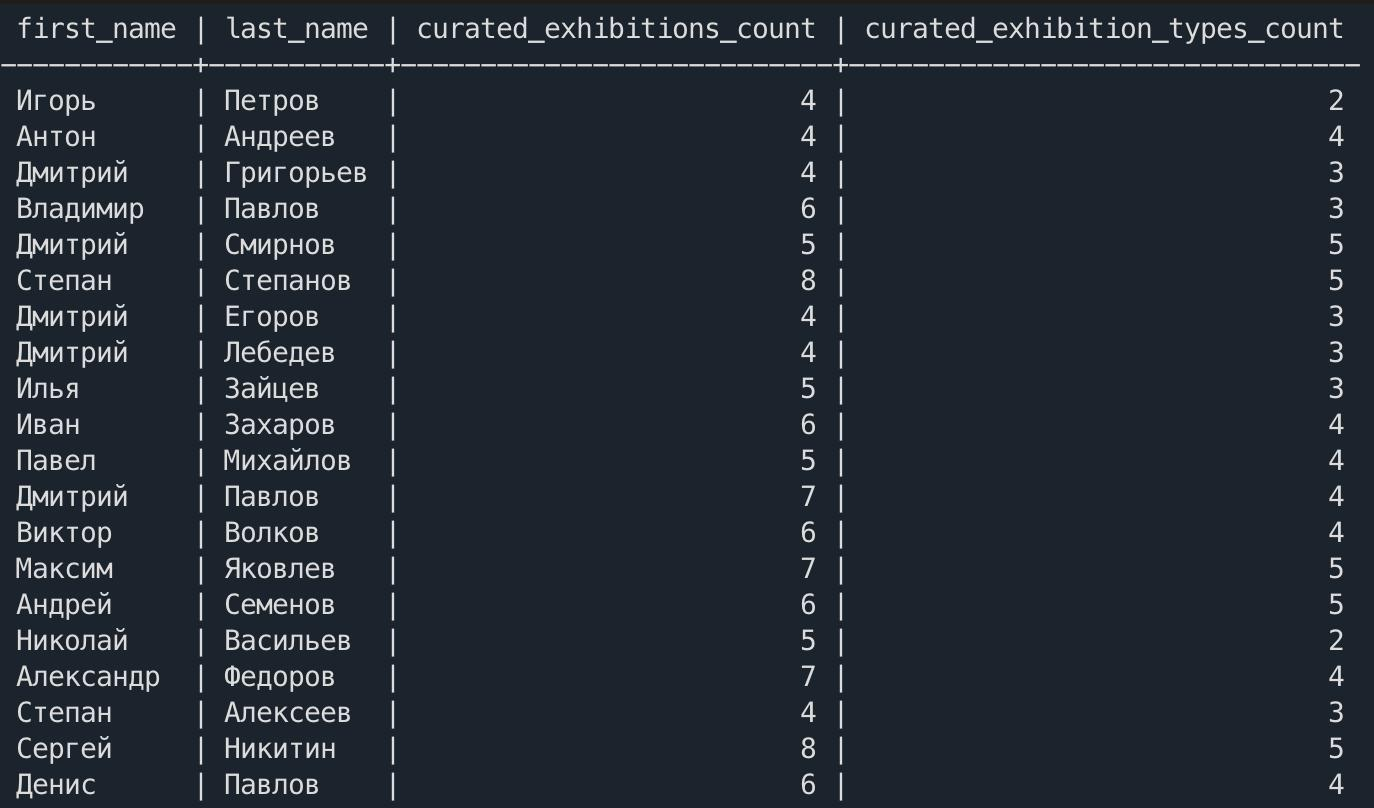
\includegraphics[width=\textwidth,height=8cm,keepaspectratio]{pic/q_view2.jpg}
    \caption{Результат выполнения простого запроса к представлению (выведены первые 20 строк)}
    \label{fig:view2-result}
\end{figure}

План выполнения запроса представлен на Рис.\ref{fig:view2-explain}. \par

\begin{figure}[H]
    \centering
    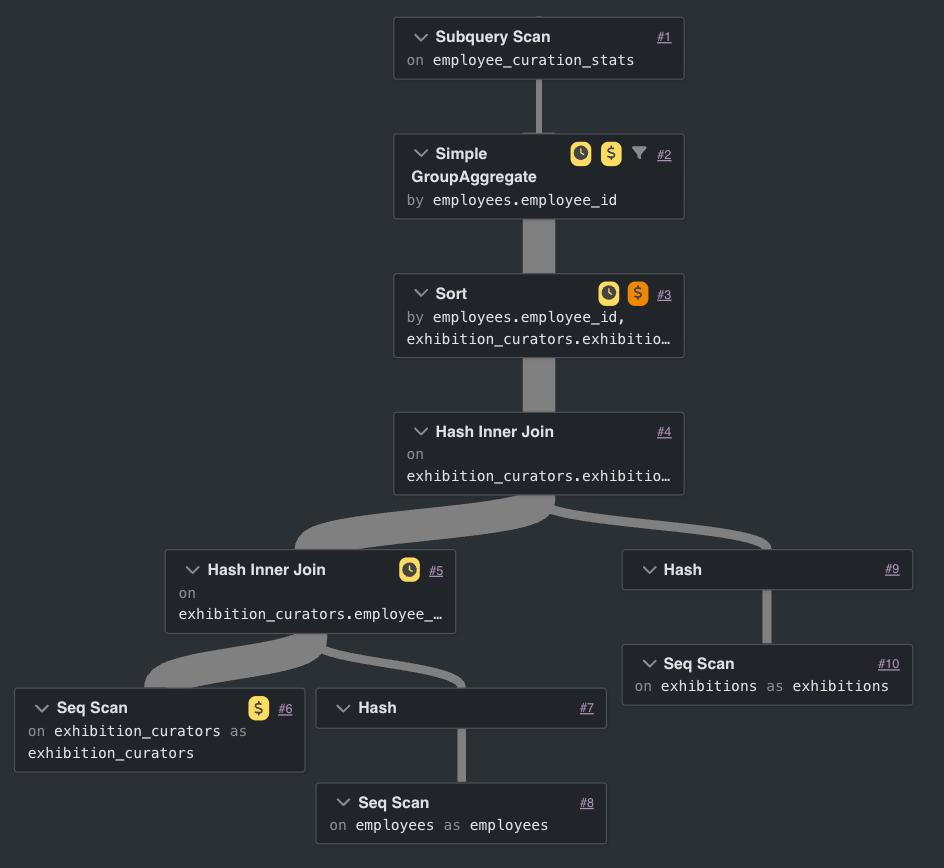
\includegraphics[width=\textwidth,height=0.75\textheight,keepaspectratio]{pic/exp_view2.jpg}
    \caption{План выполнения простого запроса к представлению}
    \label{fig:view2-explain}
\end{figure}

План разворачивает представление в подзапрос: таблицы \texttt{exhibition\_curators}, \texttt{employees} и \texttt{exhibitions} последовательно соединяются через Hash Inner Join, результат сортируется и группируется узлом Simple GroupAggregate. Условие запроса (\texttt{curated\_exhibitions\_count > 3} и \texttt{curated\_exhibition\_types\_count > 1}) планировщик применяет прямо внутри этого узла как фильтр после группировки, поэтому верхний узел Subquery Scan лишь передаёт уже отфильтрованные строки. \par

\subsection{Сложный запрос}

\textbf{Текст запроса:} Найти записи о технических паспортах, которых составили сотрудники с 2 и более курируемыми выставками. \par
Запрос соединяет (через JOIN) представление \texttt{employee\_curation\_stats} с таблицей \texttt{passports}. Текст запроса представлен в Листинге~\ref{lst:view3}. \par

\vspace{8pt}

\lstinputlisting[language=SQL, caption={Сложный запрос  с использованием представления}, label={lst:view3}, basicstyle=\ttfamily\footnotesize]{queries_view/view3.sql}

Реляционная формула запроса:
\[
\begin{gathered}
T =
\sigma_{\text{curated\_exhibitions\_count} \ \geq \ 2}
\left(
\text{passports} \ \bowtie_{\text{employee\_id}} \ \text{employee\_curation\_stats}
\right), \\
R_{view3} =
\pi_{\substack{\text{passport\_id}, \text{first\_name}, \\ \text{last\_name}, \text{curated\_exhibitions\_count}}}
\left(
T
\right), \\
\text{где } \bowtie \text{ --- это natural join}
\end{gathered}
\]

Результат выполнения запроса (выведены первые 20 строк) представлен на Рис.\ref{fig:view3-result}. \par

\begin{figure}[H]
    \centering
    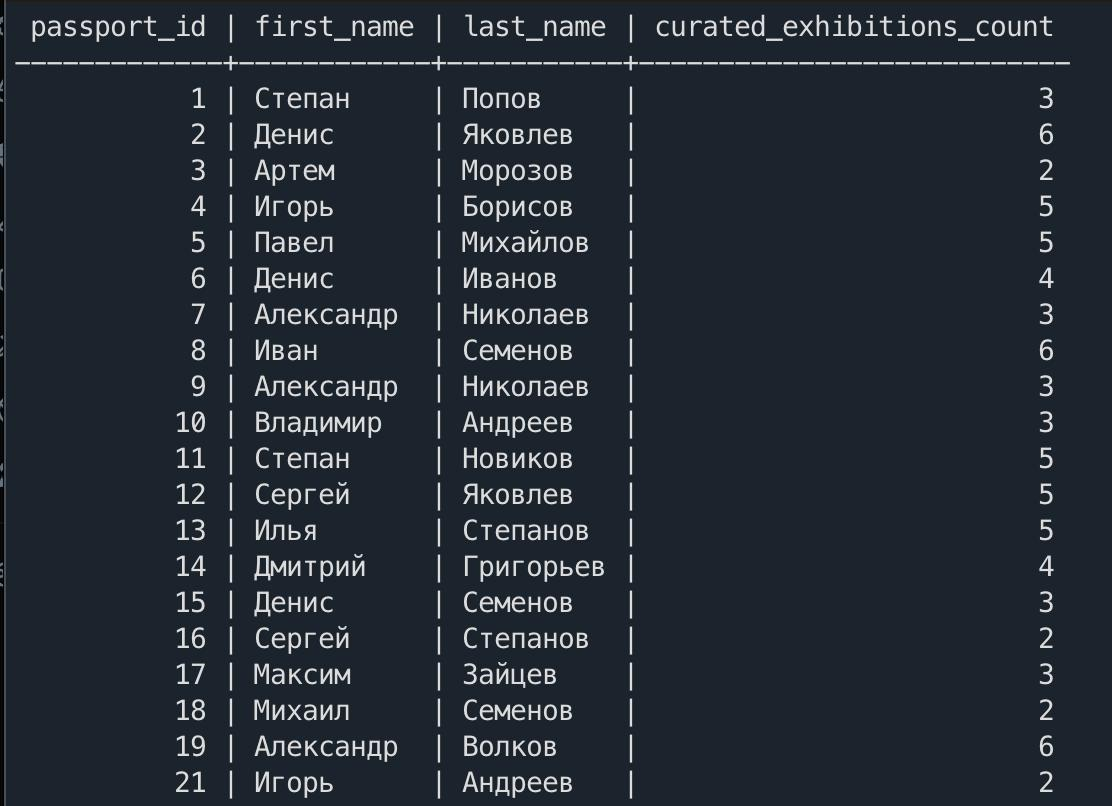
\includegraphics[width=\textwidth,height=8cm,keepaspectratio]{pic/q_view3.jpg}
    \caption{Результат выполнения сложного запроса с использованием представления (выведены первые 20 строк)}
    \label{fig:view3-result}
\end{figure}

План выполнения запроса представлен на Рис.\ref{fig:view3-explain}. \par

\begin{figure}[H]
    \centering
    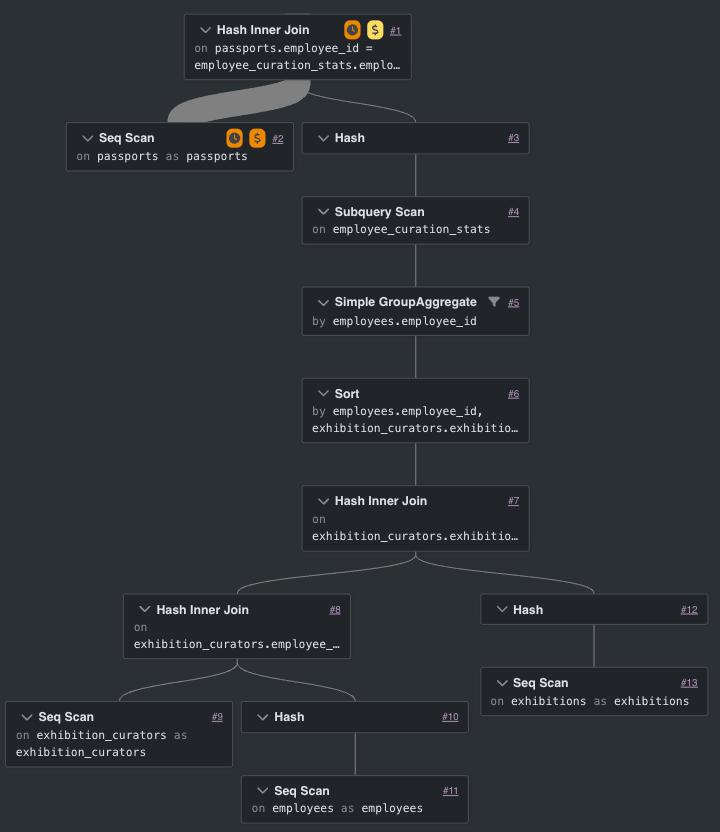
\includegraphics[width=\textwidth,height=0.75\textheight,keepaspectratio]{pic/exp_view3.jpg}
    \caption{План выполнения сложного запроса  с использованием представления}
    \label{fig:view3-explain}
\end{figure}

План аналогичен предыдущему: представление снова разворачивается в тот же набор соединений, сортировку и группировку с фильтром по числу выставок (\texttt{>= 2}). Сверху добавляется Hash Inner Join с таблицей \texttt{passports} — поскольку сторона представления после фильтрации заметно меньше (около 170 сотрудников против 300 тысяч паспортов), хэш-таблица строится именно по ней, а строки \texttt{passports} последовательно сканируются и зондируют эту таблицу. \par

\newpage
